\documentclass[10pt,aspectratio=169]{beamer}

\usepackage{iftex}
\ifPDFTeX
  \usepackage[T2A]{fontenc}
  \usepackage[utf8]{inputenc}
  \usepackage{paratype}
\else
  \usepackage{fontspec}
  \setsansfont{PT Sans}
  \setmainfont{PT Serif}
\fi
\usepackage[russian]{babel}
\usepackage{amsmath, amssymb}
\usepackage{booktabs}
\usepackage{array}
\usepackage{multirow}
\usepackage{graphicx}
\usepackage{tikz}

\usetheme{Madrid}
\setbeamertemplate{caption}[numbered]
\setbeamertemplate{bibliography item}[text]

\graphicspath{{../linearisation/literature-review/img/}}

\newcommand{\up}{\textcolor{green!50!black}}
\newcommand{\down}{\textcolor{red!70!black}}

\title[Линеаризация внимания в сегментаторах]{Линеаризация механизма внимания\texorpdfstring{\\}{ }в трансформерных сегментаторах}
\subtitle{\guillemetleft Цифровые ресурсы в научном исследовании\guillemetright}
\author[Салимли А. М.]{
  Студент: Салимли А. М., гр. 5140201/60301\texorpdfstring{\\[2pt]}{, }
  Преподаватель: к.т.н. Моторин Д. Е.}
\institute[СПбПУ]{Санкт-Петербургский политехнический университет Петра Великого\\
  Институт компьютерных наук и кибербезопасности}
\date{Санкт-Петербург, 2026}

\begin{document}

% 1
\begin{frame}
  \titlepage
\end{frame}

% 2
\begin{frame}{Содержание}
  \tableofcontents
\end{frame}

% 3
\section{Введение}
\begin{frame}{Введение}
  \begin{columns}[T]
    \begin{column}{0.55\textwidth}
      \begin{itemize}
        \item Самовнимание обеспечивает моделирование глобальных зависимостей уже на ранних стадиях сегментатора
        \item Вычислительная сложность самовнимания составляет $O(N^2)$ по числу пикселей $N$
        \item Механизм ESA в SegFormer снижает сложность лишь до $O(N^2/R)$
        \item Линеаризация направлена на достижение сложности $O(N)$ при сохранении глобального контекста
      \end{itemize}
    \end{column}
    \begin{column}{0.43\textwidth}
      \centering
      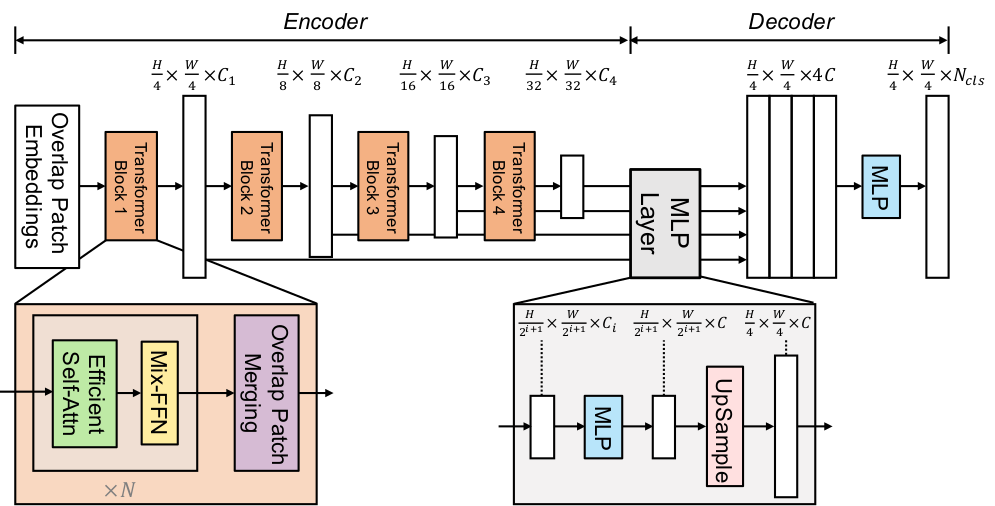
\includegraphics[width=\linewidth]{SEGFROMER_ARCH.png}\\
      {\scriptsize Архитектура SegFormer \cite{segformer}}
    \end{column}
  \end{columns}
\end{frame}

% 4
\section{Постановка проблемы}
\begin{frame}{Постановка проблемы}
  \begin{alertblock}{Общая проблема}
    Моделирование дальнего контекста требует самовнимания со сложностью $O(N^2)$, где $N = H \times W$
  \end{alertblock}
  \vspace{0.2cm}
  \centering
  \footnotesize
  \begin{tabular}{>{\raggedright\arraybackslash}p{2.6cm}>{\raggedright\arraybackslash}p{4.6cm}>{\raggedright\arraybackslash}p{3.2cm}>{\raggedright\arraybackslash}p{3.2cm}}
    \toprule
    Группа & Работы & Данные & Мера эффективности \\
    \midrule
    Сцены & SegFormer, LSNet, RTLinearFormer, HLSM-ViT & Cityscapes, ADE20K, COCO & FPS на полном кадре \\
    ДЗЗ и промышленность & GLANet, ABCFNet, LPT-Net, CA-UNet, MS-LCFNet, FESS-SAM & чаще собственные & память, FLOPs \\
    Медицина & MLFormer, MASA-VMUNet, WTP-MILA-UNet, CLT-MambaSeg, Snake-RWKV, UUEKAN, PMP & КТ, МРТ, УЗИ & параметры, FLOPs \\
    \bottomrule
  \end{tabular}
\end{frame}

% 5
\begin{frame}{Постановка проблемы: что считается узким местом}
  \begin{columns}[T]
    \begin{column}{0.5\textwidth}
      \begin{itemize}
        \item \textbf{Вычислительная сложность внимания} - LSNet, RTLinearFormer, GLANet
        \item \textbf{Деградация карты внимания} после линеаризации: ранг 71 из 128 (HLSM-ViT, UUEKAN)
        \item \textbf{Ограниченный объем выборки} - WTP-MILA-UNet, CLT-MambaSeg
        \item \textbf{Нарушение непрерывности} при развертке 2D в 1D (Snake-RWKV)
        \item \textbf{Квадратичное внимание как точка отсчета} - FESS-SAM
      \end{itemize}
    \end{column}
    \begin{column}{0.48\textwidth}
      \centering
      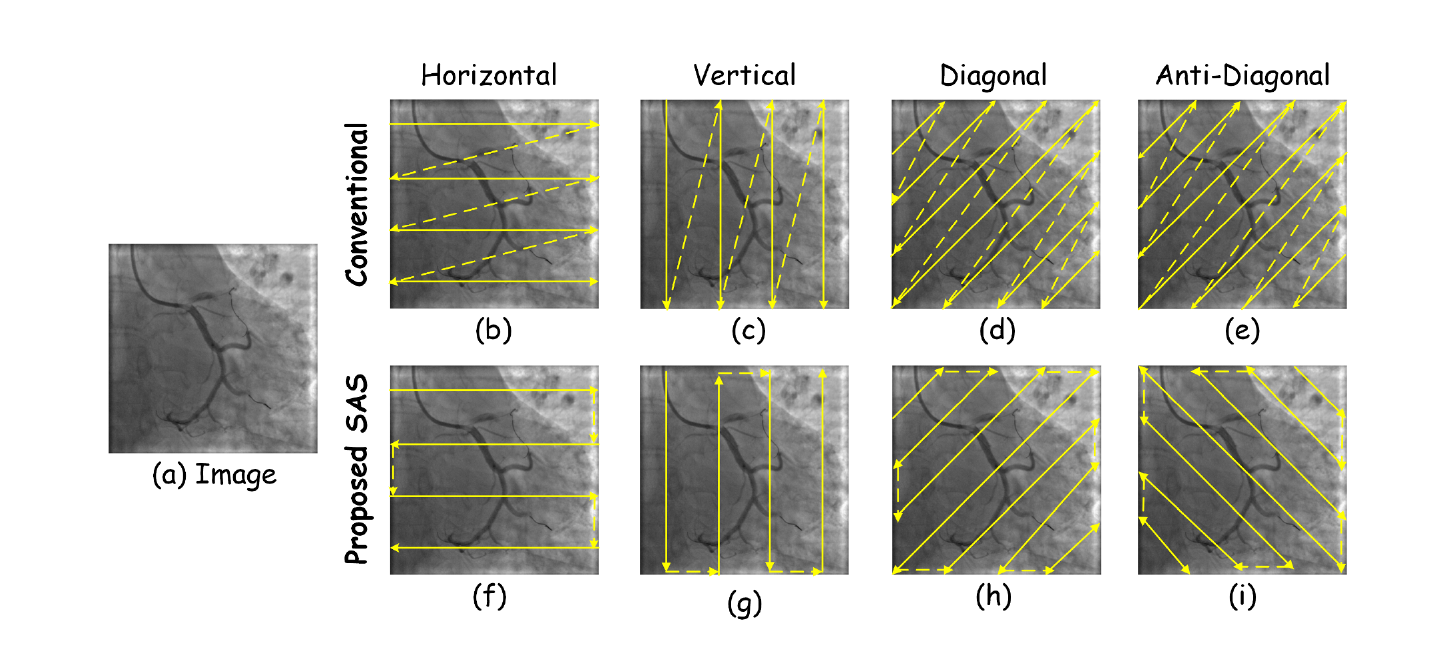
\includegraphics[width=\linewidth]{SNAKERWKV_SCAN.png}\\
      {\scriptsize Обычное и непрерывное сканирование \cite{snakerwkv}}
    \end{column}
  \end{columns}
\end{frame}

% 6
\section{Методы линеаризации}
\begin{frame}{Методы: пять семейств линеаризации}
  \centering
  \footnotesize
  \begin{tabular}{>{\raggedright\arraybackslash}p{4.4cm}>{\raggedright\arraybackslash}p{5.6cm}c}
    \toprule
    Семейство & Работы & Сложность \\
    \midrule
    Сжатие $K,V$ с softmax (ESA) & SegFormer & $O(N^2/R)$ \\
    Ядерное линейное внимание & LSNet, RTLinearFormer, GLANet, ABCFNet, MLFormer, WTP-MILA-UNet, MS-LCFNet, UUEKAN & $O(Nd^2)$ \\
    Иные приближения softmax & CLT-MambaSeg, PMP, HLSM-ViT & $O(N)$ \\
    SSM / RWKV со сканированием & MASA-VMUNet, Snake-RWKV & $O(N)$ \\
    <<Линейные>> лишь по названию & LPT-Net, CA-UNet & не по $N$ \\
    \bottomrule
  \end{tabular}
  \vspace{0.4cm}
  \begin{block}{Ядерное внимание}
    \vspace{-0.1cm}
    \[O_i = \frac{\phi(Q_i)\sum_j \phi(K_j)^T V_j}{\phi(Q_i)\sum_j \phi(K_j)^T}\]
    \vspace{-0.1cm}
  \end{block}
\end{frame}

% 7
\begin{frame}{Методы: чем дополняют линейное внимание}
  \begin{columns}[T]
    \begin{column}{0.42\textwidth}
      \begin{itemize}
        \item Размещение на глубоких стадиях с низким пространственным разрешением
        \item Сверточные ветви и гейты - RTLinearFormer, MLFormer, ABCFNet
        \item Выборочный softmax на $2\sqrt{N}$ токенах - HLSM-ViT
        \item Фокусирующее ядро - MS-LCFNet, UUEKAN
      \end{itemize}
    \end{column}
    \begin{column}{0.56\textwidth}
      \centering
      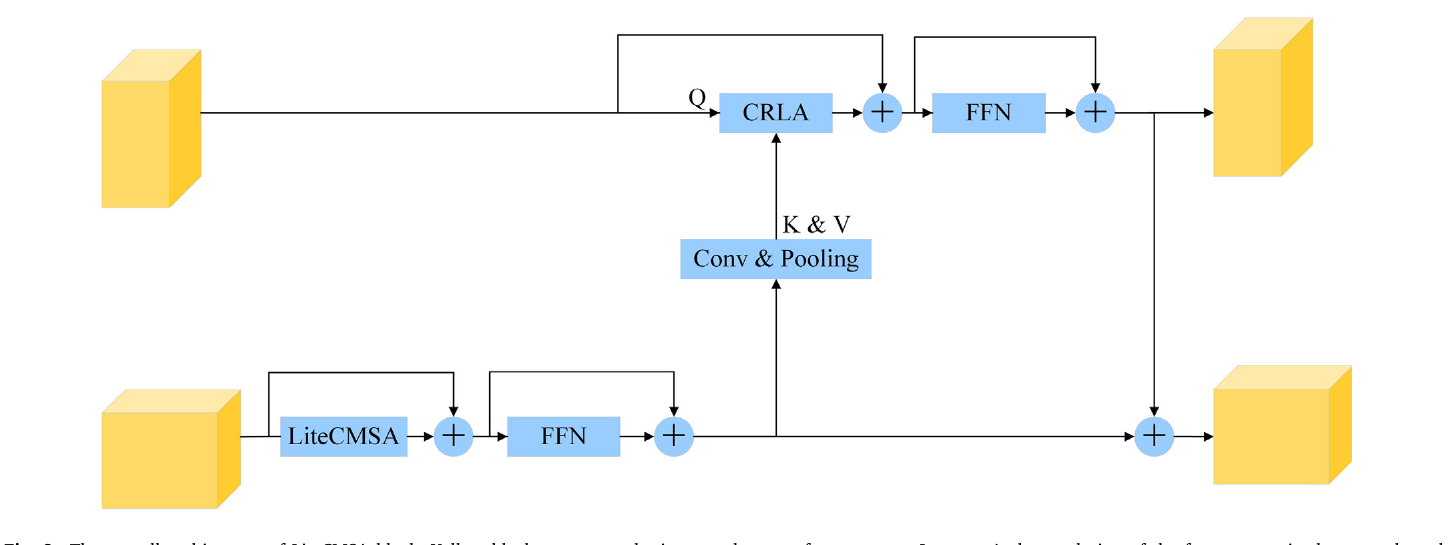
\includegraphics[width=0.75\linewidth]{RTLINEARFORMER_BLOCK.png}\\
      {\scriptsize LiteCMSA в RTLinearFormer \cite{rtlinearformer}}\\[4pt]
      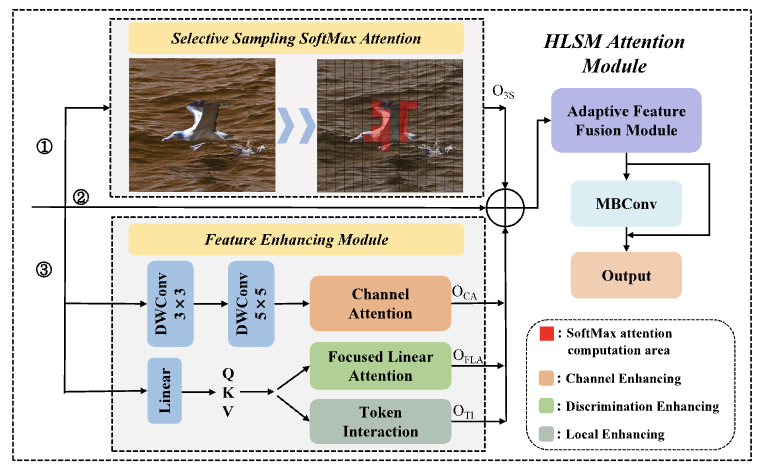
\includegraphics[width=0.55\linewidth]{HLSM_ARCH.png}\\
      {\scriptsize Гибридный модуль HLSM \cite{hlsmvit}}
    \end{column}
  \end{columns}
\end{frame}

% 8
\section{Результаты}
\begin{frame}{Результаты: линейное vs квадратичное в одной архитектуре}
  \centering
  \footnotesize
  \begin{tabular}{llcccc}
    \toprule
    Работа & Датасет, метрика & Квадр. & Линейн. & $\Delta$ качества & Стоимость \\
    \midrule
    GLANet & вход $128^2$, память & 16.5 ГБ & 44 МБ & - & \up{$\times$375 меньше} \\
    ABCFNet & Potsdam, mIoU & 87.22 & 87.48 & \up{+0.26} & \up{22 $\to$ 64 FPS} \\
    CLT-MambaSeg & ISIC-2016, IoU & 90.98 & 91.05 & \up{+0.07} & \up{8.55 $\to$ 7.02 G} \\
    MLFormer & Synapse, DSC & 77.91 & 79.24 & \up{+1.33} & \down{10.3 $\to$ 12.0 мс} \\
    RTLinearFormer & Cityscapes, mIoU & 78.86 & 78.41 & \down{$-$0.45} & \up{56 $\to$ 67 FPS} \\
    HLSM-ViT & COCO, $\mathrm{AP}^{m}$ & 32.3$^*$ & 31.2 & \down{$-$1.1} & $\approx$ \\
    \bottomrule
  \end{tabular}\\[2pt]
  {\scriptsize $^*$ гибрид с выборочным softmax}
  \vspace{0.4cm}
  \begin{itemize}
    \item На медицинских изображениях малого размера линеаризация не снижает точность
    \item На сценах высокого разрешения потеря точности составляет 0.5-1.7 п.п. mIoU
  \end{itemize}
\end{frame}

% 9
\begin{frame}{Результаты: скорость сегментаторов сцен}
  \centering
  \footnotesize
  \begin{tabular}{llllccc}
    \toprule
    Модель & Внимание & Датасет & Разрешение & mIoU & FPS & GPU \\
    \midrule
    SegFormer-B0 & ESA & Cityscapes & кор. сторона 1024 & 76.2 & 15.2 & V100 \\
    LSNet & ReLU, $O(N)$ & Cityscapes & $1024^2$ & 73.94 & \textbf{130.2} & 3080 \\
    RTLinearFormer & ReLU, $O(N)$ & Cityscapes & $1024 \times 2048$ & 78.41 & 66.7 & 3090 \\
    DDRNet-23 & нет & Cityscapes & $1024 \times 2048$ & \textbf{79.5} & 51.4 & 3090 \\
    \midrule
    SegFormer-B0 & ESA & ADE20K & $512^2$ & \textbf{37.4} & 84.4 & 3090 \\
    RTLinearFormer & ReLU, $O(N)$ & ADE20K & $512^2$ & 35.7 & \textbf{107.3} & 3090 \\
    \bottomrule
  \end{tabular}
  \vspace{0.5cm}
  \begin{block}{Вывод}
    Замена ESA линейным вниманием обеспечивает ускорение в 1.3 раза при снижении mIoU на 1.7 п.п. (одинаковые GPU и разрешение)
  \end{block}
\end{frame}

% 10
\begin{frame}{Результаты: число операций и задержка}
  \centering
  \footnotesize
  \begin{tabular}{llccc}
    \toprule
    Модель & Механизм & FLOPs (G) & Задержка (мс) & Dice (\%) \\
    \midrule
    UNet & свертки & 160.44 & \textbf{9.26} & 78.01 \\
    TransUNet & квадратичное & 133.47 & 15.74 & 78.88 \\
    SCSegamba & Mamba & \textbf{17.75} & 44.50 & 74.17 \\
    Snake-RWKV & RWKV & 45.21 & 34.23 & \textbf{80.85} \\
    \bottomrule
  \end{tabular}\\[2pt]
  {\scriptsize Вход $512 \times 512$, четыре датасета артерий \cite{snakerwkv}}
  \vspace{0.4cm}
  \begin{itemize}
    \item Модели со сканированием уступают квадратичным по задержке при меньшем числе FLOPs
    \item Эффективность линеаризации корректно оценивать по измеренной задержке
  \end{itemize}
\end{frame}

% 11
\begin{frame}{Результаты: тонкие протяженные объекты}
  \centering
  \footnotesize
  \begin{tabular}{lcccc}
    \toprule
    Модель (тоннель) & Внимание & FLOPs (G) & FPS & Mean IoU \\
    \midrule
    UNet & нет & 13.8 & \textbf{49.5} & 0.393 \\
    SegFormer-B5 & ESA & 99.7 & 17.4 & 0.651 \\
    ViT-Adapter & квадратичное & 227.9 & 16.7 & 0.765 \\
    FESS-SAM & квадратичное & 364.6 & 4.1 & \textbf{0.819} \\
    \bottomrule
  \end{tabular}\\[2pt]
  {\scriptsize Кабели, контактный провод, трубопроводы в тоннеле метро \cite{fesssam}}
  \vspace{0.3cm}
  \begin{itemize}
    \item Ошибки линейных моделей сосредоточены на тонких структурах: столбах (RTLinearFormer), линейных объектах (LPT-Net), ветвях сосудов (Snake-RWKV)
    \item На дорогах DeepGlobe ABCFNet превосходит UNet++ лишь на 0.3 п.п. IoU
  \end{itemize}
\end{frame}

% 12
\begin{frame}{Результаты: сопоставимость результатов различных работ}
  \centering
  \footnotesize
  \begin{tabular}{llccc}
    \toprule
    Модель & Механизм & Synapse (MLFormer) & Synapse (MASA) & GFLOPs \\
    \midrule
    TransUNet & самовнимание & 77.48 & 77.48 & 88.91 \\
    VM-UNet & VMamba & \down{82.38} & \down{81.08} & 4.11 \\
    MLFormer & MLLA & 83.07 & - & 9.04 \\
    MASA-VMUNet & VMamba & - & \textbf{84.36} & 4.53 \\
    \bottomrule
  \end{tabular}
  \vspace{0.4cm}
  \begin{itemize}
    \item Результаты одной базовой модели расходятся на 1.3 п.п. DSC в разных статьях
    \item На BUSI значения Dice варьируются от 74.23\% до 92.32\% вследствие различных разбиений
    \item Замеры выполнены на GPU от RTX 3060 до RTX 5090, поэтому FPS несопоставимы
  \end{itemize}
\end{frame}

% 13
\section{Заключение}
\begin{frame}{Заключение}
  \begin{itemize}
    \item Критерий эффективности зависит от области: FPS (сцены), память (ДЗЗ), параметры и FLOPs (медицина)
    \item Ядерное линейное внимание является наиболее распространенным методом линеаризации
    \item Потеря точности составляет 0.5-1.7 п.п. mIoU на сценах и отсутствует на малых входах
    \item Снижение FLOPs не гарантирует снижения задержки, особенно для Mamba и RWKV
    \item Тонкие протяженные структуры остаются наиболее сложными для линейных моделей
  \end{itemize}
  \vspace{0.2cm}
  \begin{block}{Общий вывод}
    Линейное внимание эффективно в сочетании с сверточными ветвями. Либо требует внедрения информации о топологии исходных данных.
  \end{block}
\end{frame}

\begin{frame}[plain]
  \begin{tikzpicture}[remember picture, overlay]
    \node at (current page.center)
      {\usebeamerfont{title}\usebeamercolor[fg]{structure}\Huge Спасибо за внимание!};
    \node[anchor=south east, align=right, font=\small] at ([xshift=-0.8cm, yshift=0.6cm]current page.south east)
      {Салимли А. М.\\ \texttt{salimli.am@edu.spbstu.ru}};
  \end{tikzpicture}
\end{frame}

% 14
\section{Список литературы}
\begin{frame}[t]{Список литературы}
  \vspace{-0.2cm}
  \begin{columns}[T]
    \begin{column}{0.5\textwidth}
      \scriptsize
      \begin{thebibliography}{99}
        \bibitem{segformer} Xie E. et al. SegFormer // NeurIPS. 2021.
        \bibitem{lsnet} Sheng P. et al. LSNet // Neurocomputing. 2022.
        \bibitem{rtlinearformer} Gu Y. et al. RTLinearFormer // Neurocomputing. 2025.
        \bibitem{hlsmvit} Guan S. et al. Hybrid linear attention // Pattern Recognition. 2026.
        \bibitem{glanet} Fang Y. et al. A global linear attention network // Knowledge-Based Systems. 2026.
        \bibitem{abcfnet} Zhang Z. et al. Dimensional collaborative linear-attention network // Adv. in Space Research. 2026.
        \bibitem{lptnet} Ye T. et al. LPT-Net // Measurement. 2024.
        \bibitem{caunet} Zheng Z. et al. CA-UNet // Image and Vision Computing. 2026.
        \bibitem{mslcfnet} Yang Z. et al. Multi-scale linear cross-modal fusion // Comp. and Electr. in Agriculture. 2026.
      \end{thebibliography}
    \end{column}
    \begin{column}{0.5\textwidth}
      \scriptsize
      \begin{thebibliography}{99}
        \setcounter{enumiv}{9}
        \bibitem{fesssam} Wu H. et al. FESS-SAM // Adv. Engineering Informatics. 2025.
        \bibitem{mlformer} Liu X. et al. MLFormer // Biomed. Signal Proc. and Control. 2026.
        \bibitem{masavmunet} Wang L. et al. MASA-VMUNet // Expert Syst. with Appl. 2026.
        \bibitem{wtpmilaunet} Ge H. et al. WTP-MILA-UNet // Biomed. Signal Proc. and Control. 2026.
        \bibitem{cltmambaseg} Uppal D., Prakash S. CLT-MambaSeg // Comp. in Biology and Medicine. 2025.
        \bibitem{snakerwkv} Yu C. et al. Topology-aware linear attention // Expert Syst. with Appl. 2026.
        \bibitem{uuekan} Chen Q. et al. UUEKAN // Biomed. Signal Proc. and Control. 2026.
        \bibitem{pmp} Bai D. et al. Linear-complexity global context modeling // Expert Syst. with Appl. 2026.
      \end{thebibliography}
    \end{column}
  \end{columns}
\end{frame}

\end{document}
